\section{Brightness-Based Matching}

\paragraph*{}
Brightness-based matching evaluates possible template alignments using measures of image similarity based on the relation between the brightness of the corresponding pixels of the images being compared.

\subsection{Image Correlation and Image Difference}

\paragraph*{}
While some of the measures of image similarity have natural formulation which yields high values for well-correlated images and low values for images that differ significantly, other are easier to define conversely, as measures of difference between images. To distinguish between these two groups we will use the term \textbf{image correlation} when referring to direct measures of image similarity and \textbf{image difference} when considering measures of dissimilarity. Naturally, both are equally suitable for our needs.

\paragraph*{}
We will discuss three important measures of image similarity in the context of a simple comparison benchmark demonstrated in \reftab{ImageSimilarityMeasures}.

\begin{table}[h!]
\centering
\begin{tabular}{| m{.02\linewidth} m{.13\linewidth} m{.13\linewidth} m{.12\linewidth} m{.12\linewidth} m{.12\linewidth} | }
\hline
 & & & \textbf{ME} & \textbf{MSE} & \textbf{NCC} \\
(a) & 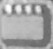
\includegraphics[width=.13\textwidth]{TemplateMatching/img/board_template} & 

\includegraphics[width=.13\textwidth]{TemplateMatching/img/board_tcomp_empty} &
54.196 & 3933.365 & 0.090 \\
(b) & 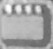
\includegraphics[width=.13\textwidth]{TemplateMatching/img/board_template} & 
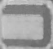
\includegraphics[width=.13\textwidth]{TemplateMatching/img/board_tcomp_detail} &
8.455 & 623.833 & 0.702 \\
(c) & 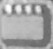
\includegraphics[width=.13\textwidth]{TemplateMatching/img/board_template} & 
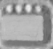
\includegraphics[width=.13\textwidth]{TemplateMatching/img/board_tcomp_another} &
10.894 & 271.555 & 0.866 \\
(d) & 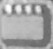
\includegraphics[width=.13\textwidth]{TemplateMatching/img/board_template} & 
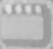
\includegraphics[width=.13\textwidth]{TemplateMatching/img/board_tcomp_linear} &
18.528 & 550.718 & 1.000 \\ \hline
\end{tabular}
\caption{Image similarity measures evaluated on example image pairs.}
\label{tab:ImageSimilarityMeasures}
\end{table}

\subsubsection{Mean Error (ME)}

\paragraph*{}
Perhaps the simplest measure of image difference is the average of its pixel-wise differences, i.e.:
\[
	\mbox{ME}(\mbox{Image}_1,\mbox{Image}_2) = \frac{1}{n} \sum_{x,y} |\mbox{Image}_1[x,y] - \mbox{Image}_2[x,y]|
\]

where $n$ denotes the number of pixels within the image dimensions.

\paragraph*{}
It is important to note that the response of this measure to a single difference depends linearly on its magnitude. This is not an optimal behavior for template matching purposes - we should use a measure that will amplify strong differences, otherwise a big number of small differences (which are inevitable due to the noise and lightning imperfections) will have impact on the result comparable with a small number of extreme differences (which should weight significantly on the score of a possible match).

\paragraph*{}
This issue may be noticed in \reftab{ImageSimilarityMeasures} examples (b) and (c). The first one yields lower mean error, even though it misses important part of the template while the second one matches the structure of the template perfectly, but contains fine differences over its entire area. 

\subsubsection{Mean Squared Error (MSE)}

\paragraph*{}
This problem is easy to address directly, by powering each term of the average:
\[
	\mbox{MSE}(\mbox{Image}_1,\mbox{Image}_2) = \frac{1}{n} \sum_{x,y} (\mbox{Image}_1[x,y] - \mbox{Image}_2[x,y])^2
\]

\paragraph*{}
Indeed, we may notice that \textbf{MSE} of the benchmark pair (c) is indeed less than half of \textbf{MSE} of (b).

\paragraph*{}
This measure is already feasible for applications in which the lightning may be relied on to be constant and uniform. Unfortunately, any change in the image brightness will heavily increase both \textbf{ME} and \textbf{MSE}. This effect may be noticed in the results for benchmark dataset (d), the second image of which is the result of linear transformation ($0.5x - 100$) of the first image.

\subsubsection{Normalized Cross-Correlation (NCC)}

\paragraph*{}
To overcome this issue we will move our attention towards an important measure of image correlation - normalized cross-correlation. 

\paragraph*{}
Normalized cross-correlation is based on an interpretation of an image as a simple one-dimensional vector of its $n$ pixel values. Such interpretation is accurate as long as we compute the image similarity pixel-by-pixel, disregarding the spatial positions of the pixels.

\paragraph*{}
For meaningful comparison of two such vectors, we need to subtract mean brightness of each image from its pixel values, thus eliminating the additive factor that would distort the proportions between individual dimensions of each vector. After such subtraction we will be left with two vectors, each having $n$ elements of the form $\mbox{Image}[i,j] - m$.

\paragraph*{}
Having eliminated the additive factor from each image, we may now deal with the multiplicative factor by normalizing each vector, i.e. by division of each element by the vector length computed as $\sqrt{\sum_{i,j} (\mbox{Image}[i,j] - m)^2}$, which happens to be the exact definition of the standard deviation $\sigma$ of the original image pixel brightness.

\paragraph*{}
Once we have reduced each image to the form of normalized, $n$-dimensional vector, we may evaluate their similarity by computing the angle $\theta$ between them. Such angle may be easily obtained, as the dot product of two normalized vectors $\mathbf{a}$ and $\mathbf{b}$ equals the cosine of the angle between them:
\[
	\cos(\theta) = \sum_{i=1}^n a_i b_i
\] 

\paragraph*{}
We may actually leave the result in the form of $\cos(\theta)$ as the cosine will conveniently scale the result to the $(-1.0, 1.0)$ range. Putting the pieces together, we obtain the formula for the normalized cross-correlation of two images:

\[
\mbox{NCC}(\mbox{Image}_1,\mbox{Image}_2) = \frac{1}{n\sigma_1 \sigma_2} \sum_{x,y} (\mbox{Image}_1[x,y]-m_1)(\mbox{Image}_2[x,y]-m_2)
\]

\paragraph*{}
The obtained method is invariant to linear changes in image brightness and proves suitable on the benchmark data set. From now on we will assume this is the method that our template matching algorithm will be based on.

\subsection{Search Procedure}

\paragraph*{}
Having selected a feasible brightness-based measure of image similarity, we may proceed to discussion of the search process itself.

\subsubsection{Template Correlation Image}

\paragraph*{}
An exhaustive search for the template occurrences is straightforward to define - we may consider each possible alignment of the template over the image and compute the normalized cross-correlation factor between the template and the part of the image that it overlaps. Results of such search may be conveniently represented on an image, each pixel of which represents the similarity factor of the template aligned over the pixel. Example \textit{template correlation image} for the input data from \reffig{TemplateMatchingBoardInput} is demonstrated in \reffig{TemplateCorrelationImage}.


\oneFigure
{TemplateMatching/img/board_correlation_image}
{Example template correlation image. Each pixel takes a value between $-1.0$ (black) and $1.0$ (white).}
{TemplateCorrelationImage}
{\basicWidth}

\paragraph*{}
Such image allows to identify the matching locations in the classic way resembling the criteria that we have used to find edge points in the \refchap{1DEdgeDetection} chapter: by extracting locally maximal points (non-maximum suppression) of magnitude greater than a predefined threshold. Example results are demonstrated in \reffig{TemplateCorrelationResults}.

\twoFigures
{TemplateMatching/img/board_correlation_maxima}
{TemplateMatching/img/board_correlation_results}
{Local maxima of the example template correlation image stronger than 0.75 on the left, corresponding matches in the original image on the right.}
{TemplateCorrelationResults}
{\basicWidth}

\subsubsection{Pyramid Matching}

\paragraph*{}
A major drawback of such simplistic search for the template occurrences lies in the computational cost of calculating the normalized cross-correlation at each location. We can trade the precision of the search for speed if we reduce the resolution of the images that we are to work with, but then we would have to face the problem of low precision, which is often equally undesirable as the problem of high processing time.

\paragraph*{}
Let us define the notion of \textit{image pyramid} as a series of images, each image being a reduced-resolution counterpart of the previous image. Usually the resolution is reduced by the factor of two in each dimension, as demonstrated in \reffig{TemplatePyramid}. The elements of image pyramid are conventionally referred to as levels, the original image being the first element at level 0.

\begin{table}[h!]
	\centering
	\tabular{c c c}
	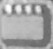
\includegraphics[width=.25\textwidth]{TemplateMatching/img/board_template_pyramid_0} &
	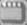
\includegraphics[width=.25\textwidth]{TemplateMatching/img/board_template_pyramid_1} &
	
\includegraphics[width=.25\textwidth]{TemplateMatching/img/board_template_pyramid_2}	

	\endtabular
	\caption{Example image pyramid.}
	\label{fig:TemplatePyramid}
\end{table}

\paragraph*{}
Pyramid matching is a technique proposed\cite{Tanimoto81} by Tanimoto, that utilizes image pyramids to combine advantages of high-precision search for template occurrences in the original images with the benefits of high-speed search in the downsampled images. 

\paragraph*{}
Pyramid search commences by computing pyramids of both the input images. The height of the pyramid is a parameter of the algorithm. It should be set to maximum value for which the template is still recognizable on the highest level of its pyramid.

\paragraph*{}
Once the image pyramids are computed, the exhaustive search for template occurrences is run using significantly downsampled images on the highest pyramid level. Similar search is then repeated at successive pyramid levels down to the original images, however on each level only the template positions that scored high on the previous level are considered.

\paragraph*{}
In this way the image areas that are unlikely to contain template occurrences are pruned from the computation on the coarse level, while promising positions are pursued through every level and in the end are identified with high precision on the original images.

\subsubsection{Multi-angle Matching}

\paragraph*{}
So far we have been assuming that the template to be identified has a fixed orientation in relation to the image axes, which is rarely the case in practice. The search process that we have described has to be therefore extended to allow for rotations of the template.

\paragraph*{}
To achieve that, we will add two additional parameters to the specification of the problem instance: a range of allowed orientations and the angular precision of the search. For instance, angle range ($-15^{\circ}$, $15^{\circ}$) and angle precision $1.0^{\circ}$ would mean that $31$ rotations of the input template shall be taken into account in the search routine. For each such rotations, separate pyramid of the template image will be computed.

\paragraph*{}
In the search procedure itself we need to identify possible match candidates using tuples of $(position, rotation)$, rather than sole positions. As such extension of the pyramid search increases the computational load roughly by the factor of the number of rotations to be considered, it is advisable to limit the range of angles being considered whenever possible (e.g. when technical conditions prevent significant deviations of the template occurrences orientation). Example results obtained using this technique are presented in \reffig{MultiAngle}

\oneFigure
{TemplateMatching/img/board_graymatching_results}
{Results on the multi-angle matching of the example data.}
{MultiAngle}
{\basicWidth}

\paragraph*{}
Similar extension may be used to match the template on multiple scales, yet such need is less common than the multi-angle matching.

\subsection{Offline Phase}

\paragraph*{}
From the above description of pyramid matching it is clear that certain amount of preprocessing is required both for the template and the search image. It is important to note, that the computational load of preprocessing for these two images is \textbf{not} equally important.

\paragraph*{}
It is extremely rare to perform template matching with one-off template - usually the template is fixed and used for inspection of a whole series of images, e.g. being captured and analyzed online. The preprocessing of the template image almost always may be performed offline and as such does not need to be the focus of possible optimizations. The results of such preprocessing along with the template image are often saved in a form of atomic datatype for easy reuse.

\paragraph*{}
The preprocessing of the search image on the other hand in most cases has to be performed online and therefore its efficiency may be crucial for the feasibility of the whole template matching-based solution. It is worth noting that the extension of the pyramid matching to multiple orientations requires computing of separate pyramids of the \textbf{template image} for every possible rotation, while the preprocessing of the search image remains limited to the calculation of a single pyramid.  

\begin{refImpl}
The measures of image similarity are implemented in \studio filters:
\begin{itemize}
	\item \filter{ImageCorrelation}{ImageMetrics}, \filter{ImageCorrelationImage}{ImageMetrics}
	\item \filter{ImageDifference}{ImageMetrics}, \filter{ImageDifferenceImage}{ImageMetrics}
\end{itemize}
First filter of each pair computes a single similarity value for two images of equal dimensions, while the second filter performs a template similarity evaluation of each possible template alignment and represents the results in form of an image, as previously described.

\paragraph*{}
Brightness-based pyramid matching is implemented in three \studio filters: \filter{CreateGrayModel}{TemplateMatching}, \filter{LocateSingleObject\_NCC}{TemplateMatching} and \filter{LocateMultipleObjects\_NCC}{TemplateMatching} - first filter performs the offline, template preprocessing phase and stores the results in atomic, reusable datatype called \textit{model}, which can be later used to perform the actual matching using the second and third filter.
\end{refImpl}